Cette section introduit les fondations théoriques de l'apprentissage par renforcement, en s'appuyant principalement sur l'ouvrage de référence de \textcite{suttonReinforcementLearningIntroduction2018} et les cours de \textcite{silverLecturesReinforcementLearning2015}.

\subsection{Le paradigme Agent-Environnement}

Le socle du RL est modélisé par une boucle d'interaction perpétuelle entre deux entités distinctes \parencite{suttonReinforcementLearningIntroduction2018} (voir Figure~\ref{fig:rl-loop}) : 
\begin{itemize}
    \item \textbf{L'agent} : le système apprenant et décisionnel.
    \item \textbf{L'environnement} : le système externe avec lequel l'agent interagit et qui réagit à ses actions.
\end{itemize}

À chaque pas de temps discret $t$, ce cycle se déroule comme suit :
\begin{enumerate}
    \item L'agent perçoit une \textbf{observation} $O_t$ de l'environnement et reçoit un signal scalaire de \textbf{récompense} $R_t$.
    \item Sur la base de ces informations, l'agent sélectionne et exécute une \textbf{action} $A_t$ dictée par sa stratégie (politique).
    \item L'environnement intègre cette action, évolue vers une nouvelle observation, puis retourne à l'agent une nouvelle observation $O_{t+1}$ ainsi qu'une récompense $R_{t+1}$ évaluant la pertinence de la transition effectuée.
\end{enumerate}

\begin{figure}[H]
\centering
\begin{tikzpicture}[
node distance=3.2cm and 5cm,
>=Stealth,
block/.style={draw, thick, minimum width=3.2cm, minimum height=1.2cm, align=center},
agent/.style={block, ellipse},
env/.style={block, rounded corners=2mm}
]

% --- Nœuds ---
\node[agent] (agent) {Agent};
\node[env, below=of agent] (env) {Environnement};

% --- Flèche Action (Droite) ---
\draw[->, thick] (agent.east) -- ++(1.5,0) |- (env.east)
node[pos=0.5, right, align=left] {action \\ $A_t$};

% --- Flèches de retour (Gauche) ---

% 1. OBSERVATION (Boucle extérieure)
\draw[->, thick] ([yshift=-0.3cm]env.west) -- ++(-3.5,0) |- ([yshift=0.2cm]agent.west);
% Label Observation (toujours à gauche de sa ligne)
\node[left, align=center] at ($(agent.west)+(-3.5, -2.2)$) {observation \\ $O_t$};
\node[below] at ($(env.west)+(-1, -0.3)$) {$O_{t+1}$};

% 2. REWARD (Boucle intérieure)
\draw[->, thick] ([yshift=0.3cm]env.west) -- ++(-3,0) |- ([yshift=-0.2cm]agent.west);
% Label REWARD déplacé à DROITE de sa ligne verticale
\node[right, align=center] at ($(agent.west)+(-3, -2.2)$) {récompense \\ $R_t$};
\node[above] at ($(env.west)+(-1, 0.3)$) {$R_{t+1}$};

% --- Ligne pointillée de transition ---
\draw[dotted, thick] ($(env.west)+(-1.5, 0.8)$) -- ($(env.west)+(-1.5, -0.8)$);

\end{tikzpicture}
\caption{Boucle d'interaction agent-environnement en apprentissage par renforcement}
\label{fig:rl-loop}
\end{figure}


\subsubsection{Exemple : Cliff Walking}

L'environnement \textit{Cliff Walking} \parencite{GymnasiumDocumentationCliffWalking} (Figure~\ref{fig:cliff-walking}) illustre ces mécanismes.
L'agent navigue sur une grille pour atteindre une cible en évitant une falaise.
Il reçoit une récompense de $-1$ par pas parcouru, afin d'inciter à emprunter le chemin le plus court, et une pénalité de $-100$ avec retour au départ s'il tombe.
Cet exemple met en évidence un compromis classique : l'agent doit trouver le chemin le plus court vers la cible tout en évitant la falaise, qui entraîne une pénalité sévère.

\begin{figure}[H]
    \centering
    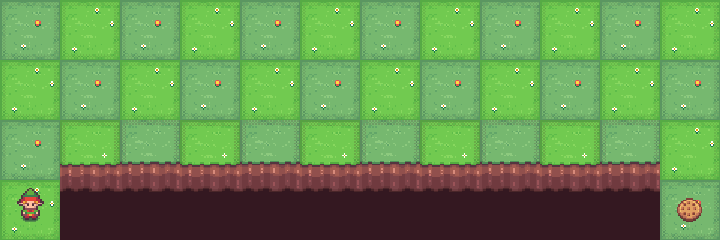
\includegraphics[width=0.6\textwidth]{img/cliff_walking.png}
    \caption{Environnement Cliff Walking.}
    \label{fig:cliff-walking}
\end{figure}

\subsection{Spécificités et Concepts Clés}


Le RL se caractérise principalement par l'absence d'expert superviseur (aucun label ne vient indiquer la "bonne" action à prendre, seul le signal de récompense sert de retour), par des signaux de récompense souvent différés, soulignant le problème de l'assignation de crédit\footnote{Problème d'assignation de crédit (\textit{Credit Assignment Problem}).}, et par des données fortement corrélées temporellement, c'est-à-dire non indépendantes et non identiquement distribuées (i.i.d.).

Afin de formaliser ce problème, voici les cinq composantes fondamentales de la boucle d'interaction \parencite{suttonReinforcementLearningIntroduction2018} :

\begin{itemize}
    \item \textbf{État de l'environnement ($S_t$)} : L'état résume l'ensemble des informations de l'environnement pertinentes à un instant $t$ pour que l'agent puisse déterminer son comportement. L'idéal est qu'il possède la \textit{propriété de Markov} (c'est-à-dire qu'il englobe tout l'historique de manière compacte).
    \item \textbf{Action ($A_t$)} : La décision exécutée par l'agent dans l'état $S_t$. Selon le problème, l'espace des actions peut être discret (par exemple : aller en haut, en bas, à gauche, à droite) ou au contraire continu (par exemple : le degré de braquage d'un volant).
    \item \textbf{Récompense ($R_{t+1}$)} : Le signal scalaire émis par l'environnement qui évalue purement et immédiatement le succès de l'action $A_t$. L'objectif central du RL est d'optimiser l'accumulation temporelle de ces retours mesurables.
    \item \textbf{Politique ($\pi$)} : La stratégie propre à l'agent. Cette fonction détermine quelles actions entreprendre en fonction de chaque état observé. Elle peut être déterministe ($a = \pi(s)$) ou stochastique, c'est-à-dire attribuer une probabilité donnée d'exécuter une action ($P(A_t = a \mid S_t = s)$).
    \item \textbf{Fonction de valeur ($V^\pi, Q^\pi$)} : Mesure la qualité (\textit{value}) d'un état (ou d'une paire état-action), c'est-à-dire l'espérance mathématique des récompenses qui seront cumulées à long terme à partir de cet état, en suivant la politique $\pi$.
\end{itemize}


\subsection{Processus Décisionnel de Markov (MDP)}
\label{sec:mdp}

L'environnement d'apprentissage dans sa globalité est formellement modélisé par un Processus Décisionnel de Markov (MDP). Ce puissant cadre mathématique repose sur la \textbf{propriété de Markov} : l'état actuel $S_t$ suffit à caractériser la dynamique future de l'environnement, indépendamment de tout l'historique passé. La prédiction de l'état suivant dépend ainsi uniquement de l'état présent, indépendamment de tout l'historique de navigation passée ($P(S_{t+1}|S_t) = P(S_{t+1}|H_t)$).

Un MDP se décrit classiquement par le système $(\mathcal{S}, \mathcal{A}, \mathcal{P}, \mathcal{R}, \gamma)$ :
\begin{itemize}
    \item $\mathcal{S}$ et $\mathcal{A}$ représentent respectivement l'ensemble des états que peut prendre l'environnement et l'ensemble des actions appartenant à l'agent.
    \item $\mathcal{P}_{ss'}^a = \mathbb{P}[S_{t+1}=s' | S_t=s, A_t=a]$ définit la matrice des probabilités de transition. Elle modélise la nature (déterministe ou probabiliste) des changements d'état résultant d'une action $a$ spécifique.
    \item $\mathcal{R}_s^a = \mathbb{E}[R_{t+1} | S_t=s, A_t=a]$ fixe la récompense espérée en transitant par l'action $a$ à partir de l'état $s$.
    \item $\gamma \in [0, 1]$ est le facteur d'actualisation (\textit{discount factor}). Il quantifie l'intérêt lié à l'horizon temporel des récompenses : une valeur de $\gamma$ proche de 0 réduit le temps de vue et favorise les gains très immédiats, tandis qu'une valeur se rapprochant de 1 insiste sur la conception de stratégies à long terme.
\end{itemize}

L'agent vise in fine à maximiser son \textbf{retour cumulé} global $G_t$, exprimé comme une somme actualisée de ces récompenses :
\begin{equation}
    G_t = R_{t+1} + \gamma R_{t+2} + \gamma^2 R_{t+3} + \dots = \sum_{k=0}^{\infty} \gamma^k R_{t+k+1}
    \label{eq:return}
\end{equation}

Pour l'exemple de \text{Cliff Walking}, on pourrait imaginer une récompense $\mathcal{R}$ de -1 par étape de déplacement (pour pénaliser le temps perdu) et de +10 en trouvant la sortie, chaque case constituant un état $\mathcal{S}$, et les pas (Gauche, Droite, Haut, Bas) constituant les actions $\mathcal{A}$. Le facteur $\gamma$ garantit alors que l'agent privilégiera mathématiquement un chemin court et rapide vers la sortie plutôt qu'une errance prolongée.


\subsection{Model-Based}
\label{sec:model-based}

Pour classifier les méthodes d'apprentissage par renforcement, il est utile de distinguer les approches basées sur un modèle (model-based) de celles sans modèle (model-free). Les méthodes model-based supposent que l'agent possède une connaissance complète de la dynamique de 
l'environnement, représentée par les fonctions de transition $P$ et de récompense $R$ (Section~\ref{sec:mdp}). Grâce à cette connaissance, l'agent peut planifier ses actions en évaluant mentalement leurs conséquences avant même de les exécuter, par des méthodes classiques de programmation dynamique telles que la Policy Iteration et la Value Iteration \parencite{suttonReinforcementLearningIntroduction2018}. Ces méthodes, bien qu'elles ne soient pas mobilisées dans les expérimentations menées dans ce travail -- centrées sur des environnements dont la dynamique n'est pas connue à l'avance --, constituent un jalon historique du domaine et permettent d'introduire par contraste les méthodes model-free développées en Section~\ref{sec:model-free}.

\subsection{Model-Free}
\label{sec:model-free}
Cependant, l'utilisation de l'apprentissage par renforcement s'applique majoritairement à des environnements réels complexes où les règles du monde sont stochastiques, inconnues, ou trop volumineuses pour être modélisées. Sans la connaissance des formules de probabilité de transition $\mathcal{P}$ ni des fonctions de récompense $\mathcal{R}$, les méthodes \textit{model-based} s'avèrent inapplicables car l'agent ne peut pas se projeter mathématiquement.

Pour surmonter cet obstacle, les méthodes dites \textit{model-free} (sans modèle) effectuent un apprentissage fondé sur l'expérience. Elles s'alimentent exclusivement des données rencontrées au cours de l'interaction de l'agent avec l'environnement pour estimer peu à peu la valeur des actions. Ce changement d'approche correspond à l'idée exprimée par \textcite{silverLecturesReinforcementLearning2015} caractérisant ces processus comme une étape de véritable apprentissage par expérience (\textit{learning}) plutôt que de simple planification en amont (\textit{planning}).

\subsubsection{Monte-Carlo}

L'approche de \textit{Monte-Carlo} (MC) \parencite{suttonReinforcementLearningIntroduction2018} s'appuie sur une idée très intuitive en ce qui concerne l'apprentissage basé sur l'expérience : la valeur d'un état correspond simplement à la moyenne de la somme des récompenses accumulées lors des passages par cet état. À l'inverse des méthodes \textit{Temporal Difference} (\textit{TD}) (voir Section \ref{sec:td}), qui mettent à jour les estimations en s'appuyant sur d'autres estimations de valeurs (créant ainsi une chaîne de prédictions imbriquées), Monte-Carlo se fie uniquement aux résultats complets observés directement sans dépendre d'approximations intermédiaires.


Le fonctionnement de base des méthodes de Monte-Carlo repose sur trois prérequis. Le premier est la nécessité de générer un apprentissage par une séquence d'expériences (états, actions, et récompenses) accumulée par l'agent au cours de ses essais successifs.
Par corrélation, l'environnement étudié doit obligatoirement être de nature "épisodique". C'est-à-dire qu'une interaction doit toujours avoir une fin déterminée, au contraire de processus cycliques tournant infiniment. En effet, tout le principe repose sur le fait de pouvoir calculer le retour accumulé et total de la session, ce qui requiert d'atteindre la fin de l'épisode (au \textit{game over} d'une partie d'échecs par exemple) pour être possible. Naturellement, ces données servent une estimation qui, répétée pour chaque nouvel essai, s'affine statistiquement au fil de l'augmentation du nombre de lancers.

Pour des raisons d'efficacité, l'algorithme ne garde pas en mémoire l'intégralité des résultats passés pour calculer sa moyenne de zéro à chaque fois. Il utilise plutôt une méthode de mise à jour incrémentale. À la fin de chaque épisode, il passe en revue les états qu'il a visités et corrige directement sa dernière estimation :

\begin{equation}
    V(S_t) \leftarrow V(S_t) + \alpha \left( G_t - V(S_t) \right)
\end{equation}

Ici, la différence $(G_t - V(S_t))$ exprime très exactement l'erreur mesurée entre le résultat du retour nouvellement calculé en finissant l'épisode ($G_t$) et l'estimation jusqu'alors théorisée pour l'état en passe d'être mis à jour ($V(S_t)$). Cette erreur est tempérée par un coefficient $\alpha$, le taux d'apprentissage (\textit{learning rate}), ce qui évite un bouleversement complet des connaissances en cas de coup de chance et lisse l'apprentissage.

Au cours d'un épisode, un état précis peut faire l'objet de visites répétées (comme l'agent passant par une case du labyrinthe plusieurs fois de suite). Ce détail force l'approche de l'algorithme à privilégier deux méthodes de traitement distinctes. Avec le premier traitement (\textit{First-Visit}), l'algorithme relève seulement et ajuste la valeur basée sur ce qui s'est déroulé après avoir touché l'état la toute première fois au cours d'une occurrence. La méthode alternative (\textit{Every-Visit}) reconsidère l'évaluation de l'état pour chacune de ses apparitions.

Si cette méthode présente l'avantage d'être très robuste (ses estimations sont toujours basées sur des résultats réels et ne sont donc pas perturbées par de potentielles prédictions erronées sur d'autres états), elle souffre cependant de défauts majeurs dans son rythme d'apprentissage. En effet, l'agent doit systématiquement attendre la fin définitive de l'épisode pour mettre à jour ses connaissances, ce qui rend la progression particulièrement lente selon l'environnement. De plus, cela crée un problème critique de forte variance : un coup de chance exceptionnel ou un désastre va impacter le score final de tout l'épisode. Cela peut conduire à des mises à jour très versatiles et irrégulières, rendant l'apprentissage instable et difficile à maîtriser.

\subsubsection{Temporal-Difference (TD)}
\label{sec:td}

Les méthodes des différences temporelles (TD) combinent les forces des méthodes de Monte-Carlo et de la programmation dynamique. À l'instar de Monte-Carlo, elles apprennent directement à partir de l'expérience brute, sans nécessiter de modèle de transition ($\mathcal{P}$). Cependant, à l'instar de la programmation dynamique, elles s'affranchissent de l'attente de la fin de l'épisode en utilisant le \textit{bootstrapping}\footnote{Principe consistant à mettre à jour l'estimation d'un état en se basant sur l'estimation de l'état suivant, plutôt que sur le retour final réel. \parencite{suttonReinforcementLearningIntroduction2018}} \parencite{suttonReinforcementLearningIntroduction2018}.

Pour illustrer cette nuance, \textcite{silverLecturesReinforcementLearning2015} propose l'analogie du trajet en voiture. Imaginons un conducteur estimant arriver chez lui à 18h30. À 18h15, il se retrouve bloqué dans un embouteillage. Une approche Monte-Carlo obligerait le conducteur à attendre d'être effectivement garé chez lui pour constater son retard et ajuster ses prévisions futures. À l'inverse, l'approche TD permet au conducteur de \textit{bootstrapper} : dès qu'il voit le bouchon, il actualise instantanément son estimation ("le trajet prendra finalement 50 minutes") sans avoir besoin de terminer sa route.

Mathématiquement, le mécanisme le plus simple, le TD(0), remplace le gain réel $G_t$ par une \textbf{cible estimée} (\textit{TD target}) composée de la récompense immédiate et de la valeur de l'état suivant :

\begin{equation}
    V(S_t) \leftarrow V(S_t) + \alpha \big( \underbrace{R_{t+1} + \gamma V(S_{t+1})}_{\text{TD target}} - V(S_t) \big)
\end{equation}

La différence entre cette cible et l'estimation actuelle est nommée \textbf{erreur TD} ($\delta_t = R_{t+1} + \gamma V(S_{t+1}) - V(S_t)$). Contrairement à Monte-Carlo, le TD(0) peut fonctionner dans des environnements continus ou cycliques car il apprend à chaque pas.

Par nature, le TD(0) ne regarde qu'un seul pas dans le futur avant de consulter son estimation. On peut toutefois généraliser ce concept en enregistrant $n$ étapes de récompenses réelles avant de \textit{bootstrapper} sur l'état $S_{t+n}$. On obtient alors le \textbf{retour à $n$ pas} (\textit{n-step return}) :

\begin{equation}
    G_t^{(n)} = R_{t+1} + \gamma R_{t+2} + \dots + \gamma^{n-1}R_{t+n} + \gamma^nV(S_{t+n})
\end{equation}

\noindent Il convient de noter que le terme de \textit{bootstrapping} $\gamma^n V(S_{t+n})$ n'est valide que si l'épisode n'est pas terminé avant l'étape $t+n$. Si l'épisode se termine à $t+k$ avec $k < n$, ce terme disparaît et le retour se réduit à la somme réelle des récompenses obtenues, ce qui équivaut à l'estimateur de Monte-Carlo.

Si $n=1$, l'approche équivaut au TD(0). Si $n \to \infty$, elle rejoint la méthode de Monte-Carlo. Le choix de $n$ devient alors un curseur permettant de modifier l'horizon de prédiction de l'agent.

Cependant, plutôt que de choisir arbitrairement ce nombre de pas ($n=1, 2, \dots, \infty$), l'algorithme $TD(\lambda)$ propose une unification de tous ces horizons en les pondérant simultanément. Ce mélange est réalisé via une moyenne pondérée par un paramètre $\lambda \in [0, 1]$, définissant ainsi le \textbf{$\lambda$-return} ($G_t^\lambda$) :

\begin{equation}
    G_t^\lambda = (1-\lambda) \sum^\infty_{n=1} \lambda^{n-1}G_t^{(n)}
\end{equation}

Bien que le $G_t^\lambda$ offre une cible robuste, il souffre du même défaut que Monte-Carlo : il regarde vers le futur et nécessite d'attendre la fin de l'épisode pour être calculé (approche dite \textit{Forward View}). Pour rendre l'apprentissage possible en temps réel, on adopte une approche \textit{Backward View} s'appuyant sur les \textbf{traces d'éligibilité} $E_t(s)$ \parencite{silverLecturesReinforcementLearning2015}.

L'équivalence mathématique entre ces deux visions permet de ne plus utiliser directement le $\lambda$-return dans la mise à jour, mais de propager l'erreur TD locale ($\delta_t$) vers le passé. Chaque état visité laisse une "empreinte" qui s'estompe avec le temps selon le facteur $\lambda$\footnote{Le paramètre $\lambda$ contrôle la persistance de la trace : une valeur proche de 0 restreint la mise à jour aux états les plus immédiats (approche "myope"), tandis qu'une valeur proche de 1 maintient l'empreinte des états anciens plus longtemps.}. La mise à jour de la trace d'éligibilité pour chaque état $s$ à chaque pas de temps $t$ s'écrit ainsi :

\begin{equation}
    E_t(s) = \gamma\lambda E_{t-1}(s) + 1(S_t = s)
\end{equation}

Ainsi, à chaque pas de temps, la fonction de valeur de \textbf{tous les états} est ajustée proportionnellement à leur responsabilité dans l'erreur courante :

\begin{equation}
    V(s) \leftarrow V(s) + \alpha \delta_t E_t(s)
\end{equation}

Cette mécanique est particulièrement efficace : dans un jeu vidéo, si un agent saute sur plusieurs plateformes avant de tomber dans un piège, le $TD(\lambda)$ permettra de baisser instantanément la valeur de toutes les plateformes de la séquence (beaucoup pour la dernière, un peu moins pour les précédentes) au prorata de leur responsabilité dans l'issue finale.

\subsection{Apprentissage en environnement inconnu}

Le passage de l'évaluation à l'optimisation consiste à améliorer la politique de l'agent sans connaissance préalable de la dynamique de l'environnement. Dans ce contexte \textit{model-free}, l'utilisation de la fonction de valeur d'état $V(s)$ s'avère insuffisante : pour choisir l'action optimale, l'agent aurait besoin de connaître les probabilités de transition $\mathcal{P}$. Par conséquent, les algorithmes de contrôle se basent sur la fonction action-valeur $Q(s,a)$, permettant d'identifier directement l'action maximisant le gain attendu \parencite{silverLecturesReinforcementLearning2015}.

\subsubsection{On-Policy vs Off-Policy}

Deux paradigmes fondamentaux s'opposent dans l'apprentissage sans modèle : 
\begin{itemize}

    \item \textbf{On-Policy} : L'agent évalue et améliore directement la politique qu'il exécute. Les expériences utilisées pour la mise à jour reflètent ses propres décisions, y compris ses stratégies d'exploration.
    \item \textbf{Off-Policy} : L'agent optimise une politique cible $\pi$ en s'appuyant sur des données générées par une politique de comportement distincte $\mu$. Cette séparation permet d'utiliser des expériences collectées par d'autres politiques pour l'apprentissage \parencite{suttonReinforcementLearningIntroduction2018}.
\end{itemize}

\subsubsection{Le dilemme Exploration-Exploitation}

Pour garantir la convergence vers une solution idéale, l'agent ne peut se contenter d'être \textit{greedy} dès le départ, au risque de rester piégé dans un optimum local. Il doit arbitrer entre l'exploitation de ses connaissances actuelles (issues de l'évaluation) et l'exploration de nouvelles stratégies. La méthode la plus répandue est la stratégie \textbf{$\epsilon$-greedy} :

\begin{equation}
\pi(a|s) = 
\begin{cases} 
1 - \epsilon + \frac{\epsilon}{m} & \text{si } a = \text{argmax}_{a \in \mathcal{A}} Q(s,a) \\
\frac{\epsilon}{m} & \text{sinon}
\end{cases}
\end{equation}

En pratique, on utilise une fonction de décroissance de $\epsilon$ (\textit{scheduler}) pour réduire progressivement sa valeur au fil du temps. Cette décroissance permet de satisfaire les conditions \textbf{GLIE}\footnote{\textit{Greedy in the Limit with Infinite Exploration}} : l'agent explore massivement au début, puis stabilise son comportement vers une politique déterministe optimale une fois l'espace état-action suffisamment parcouru. Ces conditions sont importantes car elles constituent une garantie théorique de convergence~: à condition que chaque paire état-action soit visitée un nombre infini de fois et que la politique devienne progressivement gloutonne, les algorithmes de contrôle comme SARSA sont assurés de converger vers la politique optimale $\pi^*$ \parencite{singhConvergenceResultsSingleStep2000}. Cependant, un \textit{epsilon} qui descendrait trop vite à 0 créerait un manque d'exploration, empêchant l'agent de découvrir l'intégralité des récompenses et biaisant l'optimisation.

\subsubsection{SARSA}

L'algorithme \textbf{SARSA} \parencite{suttonReinforcementLearningIntroduction2018} est une méthode d'optimisation \textbf{On-Policy}. Il met à jour la fonction $Q$ en utilisant la récompense immédiate et l'évaluation de l'action suivante ($A'$) effectivement choisie par la politique actuelle de l'agent. Son nom illustre d'ailleurs la séquence $(S, A, R, S', A')$ utilisée pour la mise à jour :
\begin{equation}
Q(S,A) \leftarrow Q(S,A) + \alpha \big( R + \gamma Q(S',A') - Q(S,A) \big)
\end{equation}

Parce qu'il inclut l'action réelle $A'$ de l'agent (et donc les erreurs potentielles liées à l'exploration) dans son calcul, SARSA réalise une optimisation "prudente". Il évalue les zones de l'environnement en tenant compte du fait qu'un mouvement aléatoire dû à $\epsilon$ pourrait entraîner une chute brutale de la récompense \parencite{silverLecturesReinforcementLearning2015}.

\subsubsection{Q-Learning}

À l'inverse, le Q-Learning \parencite{watkinsQlearning1992} est une méthode d'optimisation \textbf{Off-Policy}. Il s'affranchit de l'action réellement choisie par l'agent pour la mise à jour en utilisant l'opérateur \textit{maximum}. Il optimise directement la valeur de la politique optimale, indépendamment du comportement exploratoire :
\begin{equation}
Q(S,A) \leftarrow Q(S,A) + \alpha \big( R + \gamma \max_{a'} Q(S',a') - Q(S,A) \big)
\end{equation}

Ici, par rapport à SARSA, la mise à jour se base sur l'évaluation de la meilleure action possible ($\max$), sans tenir compte de l'action $A_{t+1}$ réellement effectuée par l'agent. Cette approche permet ainsi de converger vers la politique optimale via l'équation d'optimalité de Bellman, même si l'agent continue d'explorer activement son environnement.


\subsection{Du RL Tabulaire au Deep RL}

Les méthodes tabulaires présentées précédemment, bien que robustes, se heurtent à la \textit{malédiction de la dimensionnalité}. Dans des environnements complexes (qu'il s'agisse de flux de pixels ou de vecteurs d'états continus), le nombre de paires $(s, a)$ devient trop vaste pour être stocké ou exploré exhaustivement. 

Pour surmonter cette limite, l'\textbf{approximation de fonction} est une idée centrale. L'objectif n'est plus de maintenir un tableau de valeurs exactes, mais d'apprendre une fonction paramétrée $\hat{q}(s, a, \mathbf{w}) \approx q_\pi(s, a)$\footnote{$\textbf{w}$ le vecteur de paramètres (poids) du réseau de neurones.}, capable de généraliser les connaissances acquises vers des états jamais rencontrés.

\subsubsection{Le défi de la stabilité}

Le \textit{Deep Reinforcement Learning} (DRL) exploite la puissance des réseaux de neurones profonds comme approximateurs de fonction universels. Cependant, l'intégration de ces réseaux dans une boucle d'optimisation \textit{model-free} est intrinsèquement instable. Cette instabilité est théorisée par la \textbf{Triade Mortelle} (\textit{Deadly Triad}) \parencite{suttonReinforcementLearningIntroduction2018}, qui survient lorsque trois éléments sont réunis :
\begin{itemize}
    \item \textbf{L'approximation de fonction} (utilisation de réseaux de neurones) ;
    \item \textbf{Le \textit{bootstrapping}} (mise à jour d'estimations basées sur d'autres estimations) ;
    \item \textbf{L'apprentissage Off-Policy} (utilisation de données issues de politiques antérieures).
\end{itemize}

Sous ces conditions, la convergence des algorithmes est menacée par une forte corrélation temporelle des données et une cible de calcul mouvante (le réseau tente de rattraper une valeur qu'il modifie lui-même).

\subsubsection{Deep Q-Network}
\label{sec:dqn}

L'algorithme \textbf{Deep Q-Network (DQN)} \parencite{mnihHumanlevelControlDeep2015} a marqué l'avènement du DRL en proposant deux solutions techniques majeures pour briser cette triade et stabiliser l'optimisation :

\begin{enumerate}
    \item \textbf{Experience Replay} : Au lieu d'apprendre de manière séquentielle sur la donnée immédiate, l'agent stocke ses transitions $(s, a, r, s')$ dans une mémoire de rejeu (\textit{Replay Buffer}). Il échantillonne ensuite aléatoirement des "mini-batchs" d'expériences passées pour s'entraîner. Cela casse la corrélation temporelle des trajectoires et rend l'apprentissage plus stable en se rapprochant des conditions \textit{i.i.d.} (indépendantes et identiquement distribuées) de l'apprentissage supervisé.
    \item \textbf{Target Network} : Pour éviter que la cible de mise à jour ne change à chaque itération, DQN utilise deux réseaux distincts. Un réseau \textit{online} (paramétré par $\mathbf{w}$) qui est optimisé activement, et un réseau "cible" (\textit{target}, paramétré par $\mathbf{w}^-$) dont les poids sont gelés et périodiquement synchronisés avec le premier.
\end{enumerate}

L'apprentissage s'effectue en minimisant l'erreur quadratique moyenne entre la prédiction du réseau online et la cible fournie par le réseau target via une étape de descente de gradient. La fonction de perte (\textit{loss}) s'écrit formellement :
\begin{equation}
    L(\mathbf{w}) = \mathbb{E}_{(s,a,r,s') \sim \text{Replay}} \left[ \Big(r + \gamma \max_{a'} \hat{q}(s', a', \mathbf{w}^-) - \hat{q}(s, a, \mathbf{w})\Big)^2 \right]
\end{equation}

Cette architecture permet de converger efficacement dans des environnements à large espace d'états (comme le traitement d'images/pixels de jeux vidéo). 
Il est toutefois fondamental de retenir que l'algorithme DQN est intrinsèquement restreint aux \textbf{espaces d'actions discrets}. En effet, le calcul de la cible repose sur l'évaluation de la meilleure action future via l'opérateur $\max_{a'} \hat{q}(s', a')$. Si l'espace des actions était continu, rechercher algorithmiquement le maximum global d'une fonction neuronale hautement non linéaire à chaque itération et pour chaque transition représenterait un coût informatique prohibitif.

Pour pallier cette limitation, DDPG (\textit{Deep Deterministic Policy Gradient}) \parencite{lillicrapContinuousControlDeep2015} étend les principes de DQN aux espaces continus en apprenant simultanément une politique déterministe (l'\textit{Acteur}) et une fonction de valeur (le \textit{Critique}), supprimant ainsi la nécessité de l'opérateur $\max$. DDPG constitue la fondation architecturale directe de SAC, qui en corrige les principaux problèmes de stabilité et d'exploration, comme détaillé dans la section suivante.

\subsection{Méthodes Actor-Critic}

Pour pallier l'incompatibilité de l'algorithme DQN avec les espaces d'actions continus (comme les couples moteurs de la robotique ou le pilotage de véhicules), une approche radicalement différente est exploitée : le \textbf{Gradient de Politique} (\textit{Policy Gradient}).

L'idée est de s'affranchir de la recherche de la valeur maximale des actions pour dicter le comportement. On y optimise plutôt directement les paramètres $\theta$ d'une politique stochastique $\pi_\theta(a|s)$ par montée de gradient, dans l'optique de maximiser le retour algorithmique attendu $J(\theta) = \mathbb{E}_{\pi_\theta}[G_t]$.

\subsubsection{Architecture Actor-Critic}

Les méthodes modernes de l'état de l'art fusionnent l'apprentissage de la fonction de valeur et l'optimisation directe de la politique dans une architecture hybride nommée \textbf{Actor-Critic} \parencite{suttonReinforcementLearningIntroduction2018} :
\begin{itemize}
    \item \textbf{L'Acteur} ($\pi_\theta(a|s)$) : Un réseau de neurones constituant la politique. Il décide quelle action entreprendre.
    \item \textbf{Le Critique} ($V_w(s)$ ou $Q_w(s,a)$) : Un second réseau agissant en tant qu'évaluateur. Il calcule l'\textbf{avantage} estimé d'une action, défini comme $\hat{A}(s,a) = Q(s,a) - V(s)$, qui mesure dans quelle mesure l'action choisie est meilleure ou moins bonne que le comportement moyen attendu de la politique en cet état. Soustraire $V(s)$ joue ici le rôle de référence (\textit{baseline}) : ce résultat fondamental, établi par \textcite{williamsSimpleStatisticalGradientfollowing1992}, démontre qu'une référence ne biaise pas l'estimation du gradient de politique tout en réduisant significativement sa variance. Sans cette soustraction, le signal de mise à jour de l'Acteur serait extrêmement bruité, rendant l'apprentissage instable. Le Critique offre ainsi un signal qualitatif clair et à faible variance pour guider la mise à jour de l'Acteur.
\end{itemize}

L'avantage majeur de ce duo est qu'il paramètre intrinsèquement très bien la nature des actions (discrètes ou continues). Pour un problème \textit{discret}, la couche de sortie de l'Acteur applique une fonction \textit{Softmax} définissant la probabilité de tirer chaque action de la liste. Pour un espace \textit{continu}, l'Acteur va générer non pas des actions brutes, mais les paramètres statistiques d'une loi de distribution continue (typiquement la moyenne $\mu$ et l'écart-type $\sigma$ d'une variable gaussienne), au sein de laquelle l'action réelle sera piochée aléatoirement.

% -----------------------------------------------------------------------------
\subsubsection{Proximal Policy Optimization (PPO)}
\label{sec:ppo}
% -----------------------------------------------------------------------------
 
L'algorithme \textbf{PPO} \parencite{schulmanProximalPolicyOptimization2017}
est devenu un standard industriel du RL pour son équilibre entre simplicité
d'implémentation et grande robustesse empirique.
 
\paragraph{Estimation de l'avantage via GAE.}
PPO est fréquemment combiné avec l'estimateur \textbf{GAE}
(\textit{Generalized Advantage Estimation})
\parencite{schulmanHighDimensionalContinuousControl2018}, qui généralise
le retour à $n$ pas pour l'estimation de l'avantage. Plutôt que de fixer
un horizon $n$ arbitraire, GAE calcule une moyenne pondérée exponentiellement
de toutes les erreurs TD successives, contrôlée par un paramètre
$\lambda_{\text{GAE}} \in [0,1]$ :
 
\begin{equation}
    \hat{A}_t^{\text{GAE}(\gamma,\,\lambda_{\text{GAE}})}
    = \sum_{l=0}^{\infty} (\gamma\lambda_{\text{GAE}})^l\,\delta_{t+l}
\end{equation}
 
\noindent où $\delta_t = R_{t+1} + \gamma V(S_{t+1}) - V(S_t)$ est l'erreur
TD locale. $\lambda_{\text{GAE}}$ joue le même rôle que $\lambda$ dans
$\text{TD}(\lambda)$ : une valeur proche de $0$ produit une estimation à
faible variance mais potentiellement biaisée (horizon court), tandis qu'une
valeur proche de $1$ réduit le biais au prix d'une variance plus élevée
(horizon long). Ce paramètre sera directement retrouvé lors de la
configuration expérimentale de PPO (section~\ref{sec:hparams}).
 
\paragraph{Fonction objectif écrêtée (\textit{Clipped Surrogate Objective}).}
Un problème fondamental du gradient de politique est que des mises à jour trop
importantes peuvent détruire une politique fonctionnelle de manière
irréversible. PPO sécurise l'apprentissage en introduisant une fonction
objectif \textbf{écrêtée} qui limite
strictement l'amplitude des modifications entre deux mises à jour de la
politique :
 
\begin{equation}
    \label{eq:ppo_clip}
    L^{\text{CLIP}}(\theta) = \hat{\mathbb{E}}_t \left[
        \min\!\Big(r_t(\theta)\,\hat{A}_t,\;
        \text{clip}\!\big(r_t(\theta),\,1-\varepsilon,\,1+\varepsilon\big)\,\hat{A}_t
        \Big)
    \right]
\end{equation}
 
\noindent Les trois termes de cette expression (que l'on cherche à maximiser)
s'interprètent comme suit :
\begin{itemize}
    \item $r_t(\theta) = \dfrac{\pi_\theta(a_t|s_t)}{\pi_{\theta_{\text{old}}}(a_t|s_t)}$
          est le ratio de probabilité. Il quantifie si l'action $a_t$ est plus
          ($r_t > 1$) ou moins ($r_t < 1$) probable sous la nouvelle politique
          que sous l'ancienne.
    \item $\hat{A}_t$ est l'avantage estimé par le Critique, indiquant si
          l'action s'est révélée meilleure ou pire que l'espérance de l'état.
    \item La fonction $\text{clip}$ borne ce ratio dans l'intervalle
          $[1-\varepsilon,\, 1+\varepsilon]$ (typiquement $\varepsilon = 0.2$),
          supprimant toute incitation à s'en écarter davantage.
\end{itemize}
 
L'opérateur $\min$ garantit une politique conservatrice dans les deux sens :
si une action a été bonne ($\hat{A}_t > 0$), on cherche à augmenter sa
probabilité, mais uniquement dans la limite autorisée~; si elle a été mauvaise
($\hat{A}_t < 0$), on la pénalise, là encore dans la même fenêtre bornée.
 
\paragraph{Notion de rollout et efficacité des données.}
\label{sec:rollout}
En pratique, PPO collecte un \textbf{rollout} --- une séquence de
$n$ transitions consécutives --- avant d'effectuer ses mises
à jour. Ce batch de données est exploité sur plusieurs passes d'optimisation
($n_\text{epochs}$), découpé en mini-batchs de taille $b$.
Pour un rollout de 2\,048 steps, des mini-batchs de 256 et 20 époques, PPO
effectue ainsi $\lfloor 2048/256 \rfloor \times 20 = 160$ mises à jour du
réseau par rollout. Ce mécanisme compense partiellement la
\textit{sample efficiency}\footnote{Capacité d'un modèle à acquérir une compétence ou à atteindre un bon niveau de performance en utilisant un minimum de données (ou d'exemples) d'entraînement.} structurellement limitée des méthodes
\textit{on-policy}~; néanmoins, le batch est intégralement renouvelé après chaque cycle, les données devenant non représentatives dès que la politique est modifiée \parencite{schulmanProximalPolicyOptimization2017}.
 
% -----------------------------------------------------------------------------
\subsubsection{Soft Actor-Critic (SAC)}
\label{sec:sac}
% -----------------------------------------------------------------------------
 
\textbf{SAC} \parencite{haarnojaSoftActorCriticOffPolicy2018} étend le cadre
actor-critic en intégrant l'\textbf{entropie} de la politique à la fonction
objectif. L'agent cherche à maximiser simultanément les récompenses
accumulées et l'entropie de sa politique, afin de rester
exploratoire et d'éviter une convergence prématurée vers une stratégie
sous-optimale :
 
\begin{equation}
    J(\pi) = \sum_{t=0}^{T} \mathbb{E}_{(s_t,a_t)\sim\pi}
    \Big[\,r(s_t, a_t) + \alpha\,\mathcal{H}\!\big(\pi(\cdot|s_t)\big)\,\Big]
\end{equation}
 
\noindent où $\mathcal{H}(\pi(\cdot|s_t)) = -\mathbb{E}_{a\sim\pi}[\log\pi(a|s_t)]$
est l'entropie de Shannon de la politique en l'état $s_t$, et $\alpha > 0$
est un coefficient de température pondérant l'importance relative de l'entropie.
 
\paragraph{Ajustement automatique du coefficient d'entropie.}
Le coefficient $\alpha$ peut être fixé manuellement ou ajusté automatiquement.
\textcite{haarnojaSoftActorCriticAlgorithms2019} proposent d'optimiser
$\alpha$ à chaque step de gradient pour maintenir une entropie cible
$\mathcal{H}^*$, définie par défaut comme l'opposé de la dimension de
l'espace d'action :
 
\begin{equation}
    \mathcal{H}^* = -\dim(\mathcal{A})
\end{equation}
 
Cette valeur constitue une heuristique par défaut proposée par \textcite{haarnojaSoftActorCriticAlgorithms2019}, proportionnelle à la dimension de l'espace d'action, sans justification théorique stricte reliant cette valeur à l'entropie d'une distribution particulière -- son efficacité repose avant tout sur une validation empirique dans la littérature du contrôle continu.
 
\paragraph{Reparameterization trick.}
SAC exploite le \textbf{reparameterization trick} pour rendre son
optimisation différentiable. Échantillonner directement une action aléatoire
$a \sim \pi_\theta(\cdot|s)$ est une opération non différentiable qui bloque
la rétropropagation du gradient. 
 
\paragraph{State-Dependent Exploration (SDE).}
Par défaut, SAC rééchantillonne un bruit gaussien indépendant à chaque pas de temps, produisant une exploration sans cohérence temporelle. \textcite{raffinSmoothExplorationRobotic2021} proposent le \textit{State-Dependent Exploration} (SDE) : le bruit d'exploration $\varepsilon$ est maintenu fixe sur plusieurs steps consécutifs et dépend de l'état courant via un mapping $f(s, \varepsilon)$, permettant à l'agent d'explorer des trajectoires cohérentes plutôt que des actions isolées.
 
\paragraph{Double réseau critique.}
Pour contenir le biais de surestimation des valeurs Q
(\textit{overestimation bias}) --- problème structurel des méthodes
actor-critic identifié par \textcite{fujimotoAddressingFunctionApproximation2018}
--- SAC adopte le principe du \textbf{double réseau critique} hérité de
TD3 (\textit{Twin Delayed DDPG}), l'extension de DDPG proposée par
\textcite{fujimotoAddressingFunctionApproximation2018} pour corriger ce
biais :
 
\begin{equation}
    y = r + \gamma \min_{i=1,2} Q_{\phi_i}(s', \tilde{a}')
        - \alpha\log\pi_\theta(\tilde{a}'|s'),
    \quad \tilde{a}' \sim \pi_\theta(\cdot|s')
\end{equation}
 
En prenant le minimum, on pénalise les états sur-estimés plutôt que de les
amplifier, ce qui stabilise l'apprentissage du critique et, par ricochet,
celui de l'acteur.
 
\paragraph{Soft target update.}
Contrairement à DQN qui synchronise périodiquement son réseau cible par
copie intégrale des poids, SAC adopte une mise à jour \textbf{douce}
(\textit{soft update}) à chaque step de gradient pour chacun de ses deux
réseaux cibles :
 
\begin{equation}
    \phi_{\text{cible}} \leftarrow \tau\,\phi + (1-\tau)\,\phi_{\text{cible}}
\end{equation}
 
\noindent où $\tau \ll 1$ (valeur standard : $0.005$ \parencite{haarnojaSoftActorCriticOffPolicy2018}) est le taux
d'interpolation. Cette approche produit une cible évoluant lentement et
continûment, offrant un signal d'apprentissage plus stable que les mises
à jour discrètes de DQN. C'est l'ensemble de cette architecture --- deux
critiques, deux réseaux cibles, un acteur, et le mécanisme d'entropie
adaptative --- qui explique généralement le coût computationnel structurellement plus élevé de SAC par rapport à des algorithmes n'entretenant qu'un seul réseau critique.


\subsection{Synthèse et positionnement des algorithmes étudiés}

Les trois algorithmes retenus pour cette étude ont été délibérément choisis pour couvrir des paradigmes d'apprentissage complémentaires. Le tableau~\ref{tab:algo-comparison} résume leurs caractéristiques fondamentales selon les axes de comparaison qui structureront l'analyse expérimentale.

\begin{table}[htp]
\centering

\caption{Comparaison des algorithmes DQN, PPO et SAC selon leurs caractéristiques fondamentales.}
\label{tab:algo-comparison}

\renewcommand{\arraystretch}{1.4}
\resizebox{\textwidth}{!}{%
\begin{tabular}{|l|c|c|c|}
\hline
\textbf{Critère} & \textbf{DQN} & \textbf{PPO} & \textbf{SAC} \\
\hline
Paradigme & Off-Policy & On-Policy & Off-Policy \\
\hline
Espace d'actions & Discret & Discret / Continu & Continu \\
\hline
Replay Buffer & \checkmark & $\times$ & \checkmark \\
\hline
\textit{Sample Efficiency} & Moyenne & Faible & Élevée \\
\hline
Stabilité & Moyenne & Élevée & Élevée \\
\hline
Exploration & $\epsilon$-greedy & Stochastique (distribution apprise) & Maximisation d'entropie \\

\hline
Référence fondatrice & \textcite{mnihHumanlevelControlDeep2015} & \textcite{schulmanProximalPolicyOptimization2017} & \textcite{haarnojaSoftActorCriticOffPolicy2018} \\
\hline
\end{tabular}%
}
\end{table}

\begin{flushleft}
\footnotesize
\textit{Note} --- L'exploration de PPO est intrinsèquement stochastique :
la politique paramétrise une distribution de probabilités (catégorielle en
discret, gaussienne en continu) depuis laquelle les actions sont
échantillonnées à chaque step. Contrairement à DQN, aucun mécanisme
$\varepsilon$-greedy n'est nécessaire. Le paramètre $\varepsilon$ de PPO
désigne le seuil d'écrêtage du Clipped Surrogate Objective, sans lien avec
la stratégie d'exploration.

\textit{Note sur la Sample Efficiency} --- Ce classement reflète le nombre d'interactions avec l'environnement nécessaires pour atteindre une performance donnée. DQN, bien qu'\textit{off-policy} et doté d'une mémoire de rejeu, reste pénalisé par l'instabilité de son opérateur $\max$ et l'absence de mécanisme correctif contre la surestimation des valeurs Q, ce qui limite le gain réel tiré de la réutilisation des transitions passées. PPO, à l'inverse, rejette l'intégralité de son batch de données après chaque cycle de mises à jour (voir~\ref{sec:ppo}), ce qui en fait structurellement la méthode la moins \textit{sample-efficient} des trois malgré ses multiples époques d'optimisation par rollout. SAC combine mémoire de rejeu et double critique, ce qui explique son efficacité supérieure.
\end{flushleft}


\noindent Cette diversité de paradigmes permet une comparaison expérimentale riche : DQN sert de référence tabulaire profonde, PPO représente l'approche On-Policy de l'état de l'art, et SAC incarne l'efficacité Off-Policy avec exploration intrinsèque. Leur confrontation sur des environnements Gymnasium standardisés, puis sur un environnement complexe avec \textit{reward shaping}, constituera le cœur de l'analyse empirique de ce mémoire.